
%% bare_conf.tex
%% V1.3
%% 2007/01/11
%% by Michael Shell
%% See:
%% http://www.michaelshell.org/
%% for current contact information.
%%
%% This is a skeleton file demonstrating the use of IEEEtran.cls
%% (requires IEEEtran.cls version 1.7 or later) with an IEEE conference paper.
%%
%% Support sites:
%% http://www.michaelshell.org/tex/ieeetran/
%% http://www.ctan.org/tex-archive/macros/latex/contrib/IEEEtran/
%% and
%% http://www.ieee.org/

%%*************************************************************************
%% Legal Notice:
%% This code is offered as-is without any warranty either expressed or
%% implied; without even the implied warranty of MERCHANTABILITY or
%% FITNESS FOR A PARTICULAR PURPOSE! 
%% User assumes all risk.
%% In no event shall IEEE or any contributor to this code be liable for
%% any damages or losses, including, but not limited to, incidental,
%% consequential, or any other damages, resulting from the use or misuse
%% of any information contained here.
%%
%% All comments are the opinions of their respective authors and are not
%% necessarily endorsed by the IEEE.
%%
%% This work is distributed under the LaTeX Project Public License (LPPL)
%% ( http://www.latex-project.org/ ) version 1.3, and may be freely used,
%% distributed and modified. A copy of the LPPL, version 1.3, is included
%% in the base LaTeX documentation of all distributions of LaTeX released
%% 2003/12/01 or later.
%% Retain all contribution notices and credits.
%% ** Modified files should be clearly indicated as such, including  **
%% ** renaming them and changing author support contact information. **
%%
%% File list of work: IEEEtran.cls, IEEEtran_HOWTO.pdf, bare_adv.tex,
%%                    bare_conf.tex, bare_jrnl.tex, bare_jrnl_compsoc.tex
%%*************************************************************************

% *** Authors should verify (and, if needed, correct) their LaTeX system  ***
% *** with the testflow diagnostic prior to trusting their LaTeX platform ***
% *** with production work. IEEE's font choices can trigger bugs that do  ***
% *** not appear when using other class files.                            ***
% The testflow support page is at:
% http://www.michaelshell.org/tex/testflow/



% Note that the a4paper option is mainly intended so that authors in
% countries using A4 can easily print to A4 and see how their papers will
% look in print - the typesetting of the document will not typically be
% affected with changes in paper size (but the bottom and side margins will).
% Use the testflow package mentioned above to verify correct handling of
% both paper sizes by the user's LaTeX system.
%
% Also note that the "draftcls" or "draftclsnofoot", not "draft", option
% should be used if it is desired that the figures are to be displayed in
% draft mode.
%
\documentclass[conference]{IEEEtran}
% Add the compsoc option for Computer Society conferences.
%
% If IEEEtran.cls has not been installed into the LaTeX system files,
% manually specify the path to it like:
% \documentclass[conference]{../sty/IEEEtran}
% Some very useful LaTeX packages include:
% (uncomment the ones you want to load)

% *** MISC UTILITY PACKAGES ***
%
%\usepackage{ifpdf}
% Heiko Oberdiek's ifpdf.sty is very useful if you need conditional
% compilation based on whether the output is pdf or dvi.
% usage:
% \ifpdf
%   % pdf code
% \else
%   % dvi code
% \fi
% The latest version of ifpdf.sty can be obtained from:
% http://www.ctan.org/tex-archive/macros/latex/contrib/oberdiek/
% Also, note that IEEEtran.cls V1.7 and later provides a builtin
% \ifCLASSINFOpdf conditional that works the same way.
% When switching from latex to pdflatex and vice-versa, the compiler may
% have to be run twice to clear warning/error messages.

% *** CITATION PACKAGES ***
%
\usepackage{cite}
% cite.sty was written by Donald Arseneau
% V1.6 and later of IEEEtran pre-defines the format of the cite.sty package
% \cite{} output to follow that of IEEE. Loading the cite package will
% result in citation numbers being automatically sorted and properly
% "compressed/ranged". e.g., [1], [9], [2], [7], [5], [6] without using
% cite.sty will become [1], [2], [5]--[7], [9] using cite.sty. cite.sty's
% \cite will automatically add leading space, if needed. Use cite.sty's
% noadjust option (cite.sty V3.8 and later) if you want to turn this off.
% cite.sty is already installed on most LaTeX systems. Be sure and use
% version 4.0 (2003-05-27) and later if using hyperref.sty. cite.sty does
% not currently provide for hyperlinked citations.
% The latest version can be obtained at:
% http://www.ctan.org/tex-archive/macros/latex/contrib/cite/
% The documentation is contained in the cite.sty file itself.

% *** GRAPHICS RELATED PACKAGES ***
%
\ifCLASSINFOpdf
  % \usepackage[pdftex]{graphicx}
  % declare the path(s) where your graphic files are
  % \graphicspath{{../pdf/}{../jpeg/}}
  % and their extensions so you won't have to specify these with
  % every instance of \includegraphics
  % \DeclareGraphicsExtensions{.pdf,.jpeg,.png}
\else
  % or other class option (dvipsone, dvipdf, if not using dvips). graphicx
  % will default to the driver specified in the system graphics.cfg if no
  % driver is specified.
  \usepackage[dvips]{graphicx}
  % declare the path(s) where your graphic files are
  \graphicspath{{../fig/}}
  % and their extensions so you won't have to specify these with
  % every instance of \includegraphics
  % \DeclareGraphicsExtensions{.eps}
\fi
% graphicx was written by David Carlisle and Sebastian Rahtz. It is
% required if you want graphics, photos, etc. graphicx.sty is already
% installed on most LaTeX systems. The latest version and documentation can
% be obtained at: 
% http://www.ctan.org/tex-archive/macros/latex/required/graphics/
% Another good source of documentation is "Using Imported Graphics in
% LaTeX2e" by Keith Reckdahl which can be found as epslatex.ps or
% epslatex.pdf at: http://www.ctan.org/tex-archive/info/
%
% latex, and pdflatex in dvi mode, support graphics in encapsulated
% postscript (.eps) format. pdflatex in pdf mode supports graphics
% in .pdf, .jpeg, .png and .mps (metapost) formats. Users should ensure
% that all non-photo figures use a vector format (.eps, .pdf, .mps) and
% not a bitmapped formats (.jpeg, .png). IEEE frowns on bitmapped formats
% which can result in "jaggedy"/blurry rendering of lines and letters as
% well as large increases in file sizes.
%
% You can find documentation about the pdfTeX application at:
% http://www.tug.org/applications/pdftex

% *** MATH PACKAGES ***
%
\usepackage[cmex10]{amsmath}
% A popular package from the American Mathematical Society that provides
% many useful and powerful commands for dealing with mathematics. If using
% it, be sure to load this package with the cmex10 option to ensure that
% only type 1 fonts will utilized at all point sizes. Without this option,
% it is possible that some math symbols, particularly those within
% footnotes, will be rendered in bitmap form which will result in a
% document that can not be IEEE Xplore compliant!
%
% Also, note that the amsmath package sets \interdisplaylinepenalty to 10000
% thus preventing page breaks from occurring within multiline equations. Use:
\interdisplaylinepenalty=2500
% after loading amsmath to restore such page breaks as IEEEtran.cls normally
% does. amsmath.sty is already installed on most LaTeX systems. The latest
% version and documentation can be obtained at:
% http://www.ctan.org/tex-archive/macros/latex/required/amslatex/math/

% *** SPECIALIZED LIST PACKAGES ***
%
%\usepackage{algorithmic}
% algorithmic.sty was written by Peter Williams and Rogerio Brito.
% This package provides an algorithmic environment fo describing algorithms.
% You can use the algorithmic environment in-text or within a figure
% environment to provide for a floating algorithm. Do NOT use the algorithm
% floating environment provided by algorithm.sty (by the same authors) or
% algorithm2e.sty (by Christophe Fiorio) as IEEE does not use dedicated
% algorithm float types and packages that provide these will not provide
% correct IEEE style captions. The latest version and documentation of
% algorithmic.sty can be obtained at:
% http://www.ctan.org/tex-archive/macros/latex/contrib/algorithms/
% There is also a support site at:
% http://algorithms.berlios.de/index.html
% Also of interest may be the (relatively newer and more customizable)
% algorithmicx.sty package by Szasz Janos:
% http://www.ctan.org/tex-archive/macros/latex/contrib/algorithmicx/

% *** ALIGNMENT PACKAGES ***
%
%\usepackage{array}
% Frank Mittelbach's and David Carlisle's array.sty patches and improves
% the standard LaTeX2e array and tabular environments to provide better
% appearance and additional user controls. As the default LaTeX2e table
% generation code is lacking to the point of almost being broken with
% respect to the quality of the end results, all users are strongly
% advised to use an enhanced (at the very least that provided by array.sty)
% set of table tools. array.sty is already installed on most systems. The
% latest version and documentation can be obtained at:
% http://www.ctan.org/tex-archive/macros/latex/required/tools/

%\usepackage{mdwmath}
%\usepackage{mdwtab}
% Also highly recommended is Mark Wooding's extremely powerful MDW tools,
% especially mdwmath.sty and mdwtab.sty which are used to format equations
% and tables, respectively. The MDWtools set is already installed on most
% LaTeX systems. The lastest version and documentation is available at:
% http://www.ctan.org/tex-archive/macros/latex/contrib/mdwtools/

% IEEEtran contains the IEEEeqnarray family of commands that can be used to
% generate multiline equations as well as matrices, tables, etc., of high
% quality.

%\usepackage{eqparbox}
% Also of notable interest is Scott Pakin's eqparbox package for creating
% (automatically sized) equal width boxes - aka "natural width parboxes".
% Available at:
% http://www.ctan.org/tex-archive/macros/latex/contrib/eqparbox/

% *** SUBFIGURE PACKAGES ***
\usepackage[tight,footnotesize]{subfigure}
% subfigure.sty was written by Steven Douglas Cochran. This package makes it
% easy to put subfigures in your figures. e.g., "Figure 1a and 1b". For IEEE
% work, it is a good idea to load it with the tight package option to reduce
% the amount of white space around the subfigures. subfigure.sty is already
% installed on most LaTeX systems. The latest version and documentation can
% be obtained at:
% http://www.ctan.org/tex-archive/obsolete/macros/latex/contrib/subfigure/
% subfigure.sty has been superceeded by subfig.sty.

%\usepackage[caption=false]{caption}
%\usepackage[font=footnotesize]{subfig}
% subfig.sty, also written by Steven Douglas Cochran, is the modern
% replacement for subfigure.sty. However, subfig.sty requires and
% automatically loads Axel Sommerfeldt's caption.sty which will override
% IEEEtran.cls handling of captions and this will result in nonIEEE style
% figure/table captions. To prevent this problem, be sure and preload
% caption.sty with its "caption=false" package option. This is will preserve
% IEEEtran.cls handing of captions. Version 1.3 (2005/06/28) and later 
% (recommended due to many improvements over 1.2) of subfig.sty supports
% the caption=false option directly:
%\usepackage[caption=false,font=footnotesize]{subfig}
%
% The latest version and documentation can be obtained at:
% http://www.ctan.org/tex-archive/macros/latex/contrib/subfig/
% The latest version and documentation of caption.sty can be obtained at:
% http://www.ctan.org/tex-archive/macros/latex/contrib/caption/

% *** FLOAT PACKAGES ***
%
%\usepackage{fixltx2e}
% fixltx2e, the successor to the earlier fix2col.sty, was written by
% Frank Mittelbach and David Carlisle. This package corrects a few problems
% in the LaTeX2e kernel, the most notable of which is that in current
% LaTeX2e releases, the ordering of single and double column floats is not
% guaranteed to be preserved. Thus, an unpatched LaTeX2e can allow a
% single column figure to be placed prior to an earlier double column
% figure. The latest version and documentation can be found at:
% http://www.ctan.org/tex-archive/macros/latex/base/

%\usepackage{stfloats}
% stfloats.sty was written by Sigitas Tolusis. This package gives LaTeX2e
% the ability to do double column floats at the bottom of the page as well
% as the top. (e.g., "\begin{figure*}[!b]" is not normally possible in
% LaTeX2e). It also provides a command:
%\fnbelowfloat
% to enable the placement of footnotes below bottom floats (the standard
% LaTeX2e kernel puts them above bottom floats). This is an invasive package
% which rewrites many portions of the LaTeX2e float routines. It may not work
% with other packages that modify the LaTeX2e float routines. The latest
% version and documentation can be obtained at:
% http://www.ctan.org/tex-archive/macros/latex/contrib/sttools/
% Documentation is contained in the stfloats.sty comments as well as in the
% presfull.pdf file. Do not use the stfloats baselinefloat ability as IEEE
% does not allow \baselineskip to stretch. Authors submitting work to the
% IEEE should note that IEEE rarely uses double column equations and
% that authors should try to avoid such use. Do not be tempted to use the
% cuted.sty or midfloat.sty packages (also by Sigitas Tolusis) as IEEE does
% not format its papers in such ways.

% *** PDF, URL AND HYPERLINK PACKAGES ***
%
\usepackage{url}
% url.sty was written by Donald Arseneau. It provides better support for
% handling and breaking URLs. url.sty is already installed on most LaTeX
% systems. The latest version can be obtained at:
% http://www.ctan.org/tex-archive/macros/latex/contrib/misc/
% Read the url.sty source comments for usage information. Basically,
% \url{my_url_here}.

% *** Do not adjust lengths that control margins, column widths, etc. ***
% *** Do not use packages that alter fonts (such as pslatex).         ***
% There should be no need to do such things with IEEEtran.cls V1.6 and later.
% (Unless specifically asked to do so by the journal or conference you plan
% to submit to, of course. )

\usepackage{multirow}
\usepackage{tikz}

% correct bad hyphenation here
\hyphenation{op-tical net-works semi-conduc-tor}

\newcommand{\eqdef}{\overset{\mathrm{def}}{=\joinrel=}}

%\linespread{2}

\begin{document}
%
% paper title
% can use linebreaks \\ within to get better formatting as desired
\title{Real-Time Continuous Gesture Recognition for Natural Human-Computer
Interaction }

% author names and affiliations
% use a multiple column layout for up to three different
% affiliations
\author{\IEEEauthorblockN{Ying Yin}
\IEEEauthorblockA{CSAIL MIT\\
Email: yingyin@csail.mit.edu}
\and
\IEEEauthorblockN{Randall Davis}
\IEEEauthorblockA{CSAIL MIT\\
Email: davis@csail.mit.edu}
}

% conference papers do not typically use \thanks and this command
% is locked out in conference mode. If really needed, such as for
% the acknowledgment of grants, issue a \IEEEoverridecommandlockouts
% after \documentclass

% for over three affiliations, or if they all won't fit within the width
% of the page, use this alternative format:
% 
%\author{\IEEEauthorblockN{Michael Shell\IEEEauthorrefmark{1},
%Homer Simpson\IEEEauthorrefmark{2},
%James Kirk\IEEEauthorrefmark{3}, 
%Montgomery Scott\IEEEauthorrefmark{3} and
%Eldon Tyrell\IEEEauthorrefmark{4}}
%\IEEEauthorblockA{\IEEEauthorrefmark{1}School of Electrical and Computer Engineering\\
%Georgia Institute of Technology,
%Atlanta, Georgia 30332--0250\\ Email: see http://www.michaelshell.org/contact.html}
%\IEEEauthorblockA{\IEEEauthorrefmark{2}Twentieth Century Fox, Springfield, USA\\
%Email: homer@thesimpsons.com}
%\IEEEauthorblockA{\IEEEauthorrefmark{3}Starfleet Academy, San Francisco, California 96678-2391\\
%Telephone: (800) 555--1212, Fax: (888) 555--1212}
%\IEEEauthorblockA{\IEEEauthorrefmark{4}Tyrell Inc., 123 Replicant Street, Los Angeles, California 90210--4321}}

% make the title area
\maketitle

\begin{abstract}
%\boldmath
Our real-time continuous gesture recognition system addresses problems that
have previously been neglected: handling both gestures that are
characterized by distinct paths and gestures characterized by distinct hand
poses; and determining how and when the system should respond to gestures. Our probabilistic 
recognition framework based on hidden
Markov models (HMMs) unifies the recognition of the two forms of gestures.
Using information from the
hidden states in the HMM, we can identify different
gesture phases: the pre-stroke, the nucleus and the post-stroke
phases.
This allows the system to respond appropriately to both gestures that
require a discrete response and those needing a continuous response.
Our system is extensible: in only a few minutes, users can define their own
gestures by giving a few examples rather than writing code.
We also collected a new gesture dataset that
contains the two forms of gestures, and propose a new hybrid performance
metric for evaluating gesture recognition methods for real-time
interaction.

\end{abstract}
% IEEEtran.cls defaults to using nonbold math in the Abstract.
% This preserves the distinction between vectors and scalars. However,
% if the conference you are submitting to favors bold math in the abstract,
% then you can use LaTeX's standard command \boldmath at the very start
% of the abstract to achieve this. Many IEEE journals/conferences frown on
% math in the abstract anyway.

\begin{IEEEkeywords}
Gesture recognition, real-time, hidden Markov models
\end{IEEEkeywords}

% For peer review papers, you can put extra information on the cover
% page as needed:
% \ifCLASSOPTIONpeerreview
% \begin{center} \bfseries EDICS Category: 3-BBND \end{center}
% \fi
%
% For peerreview papers, this IEEEtran command inserts a page break and
% creates the second title. It will be ignored for other modes.
\IEEEpeerreviewmaketitle

\section{Introduction}
% no \IEEEPARstart
\begin{quotation}
Imagine how nice it would be, the next time you make a presentation, you do
not need to stand close to your laptop or use a remote control with limited
functionality. What if you could present your work as naturally as having a
conversation with your audience. You swipe your hand left and right to change slides. When you point to the slide
with your hand, the display shows a pointer cursor following where you are
pointing at. When you are showing a video,
you use a palm forward hand pose and move left and right to fast forward or
rewind the video. 
When you need to jump to a particular slide, you make a circle
gesture to show all the slides, and say ``show this
slide'' while pointing at that slide. You can also make a dismiss gesture to
pause the slide show (making the screen black) to 
get full attention from the audience.
\end{quotation}

This scenario shows an application of multi-modal interface to a
real-world problem. Different categories of gestures play an important part in
the scenario. 

Gestural input has just become popular recently with the introduction
of new sensors (e.g. Kinect, Leap). As gesture recognition systems mature,
gestural input will become an integral part of human computer interfaces, and
hence will be an interesting area to explore in terms of visual languages.

Many gesture input interfaces still mainly make the hands function as a
mouse with a limited number of other gestures. 
Previous research on gesture
recognition usually focuses on one category of gestures, and the evaluation is
also based on offline recognition.
 We believe that to design a gesture
recognition system for natural human computer interaction (HCI), we need to
start from the user interaction perspective:
what are the different categories of gestures people use;
when should the system respond; and how should the model be trained or defined.
These are the questions we addressed when we develop our system.

The main contributions of this work include:
\begin{itemize}
  \item We developed a unified probabilistic framework for real-time gesture
  recognition that combines two forms of gestures.
  \item We use embedded training and hidden state information to detect
  different gesture phases, allowing the system to respond more promptly.
  \item We collected a new dataset that include two forms of gestures, a
  combination currently lacking in the community. We also propose a hybrid
  evaluation metric that is more relevant to real-time interaction and different
  categories of gestures.
\end{itemize}

\section{Gesture Taxonomy for Natural Interaction}\label{sec:taxonomy}
This section introduces important
concepts in gesture taxonomy that are the basis of our gesture modeling.
Several gesture taxonomies have been suggested in the literature
\cite{kendon86, Pavlovic97}, but the one that seems most appropriate for natural
HCI and human-centric design was developed Wobbrock et al. \cite{wobbrock09}. Their
study is based on eliciting natural behavior from non-technical users when
interacting with a computing system. 

Wobbrock et al. classify gestures in four orthogonal dimensions. As a first
step, we focus on two of them (Table~\ref{tab:taxonomy}) and incorporate them in
designing the gesture recognition system and interface. We also further generalize the
taxonomy to encompass interaction for both vertical and horizontal displays.

\subsection{Gesture Forms and Flows}
One dimension is the \textit{form} of a gesture; we distinguish two
categories in this dimension: path and pose. The path category 
contains gestures characterized by distinct paths without any distinct
hand pose. For example, a ``swipe left'' gesture is characterized by a
right to left motion, while a ``circle'' gesture is characterized by a
circular motion of the hand. In doing these, users typically hold their
hands in some natural relaxed pose. The second category of gestures is
characterized by distinct hand poses without any distinct paths. This category
of gestures is usually associated with direct manipulation of some virtual
objects on the interface.
For example, a user may use a ``point'' hand pose and move around to
point at different things on a display.

\begin{table}[t]
\caption{Taxonomy of gestures for natural interaction.}
\label{tab:taxonomy}
\centering
\begin{tabular}{|c|l|l|}
\hline
\multirow{2}{*}{\textbf{\textit{Form}}} & \textit{distinct path} & with any hand
pose
\\
\cline{2-3} 
                               & \textit{distinct hand pose} & with any path \\
\hline
\multirow{2}{*}{\textbf{\textit{Flow}}} & \textit{discrete} & response occurs
\textit{after} the user acts \\
\cline{2-3}
              & \textit{continuous} & response occurs \textit{while} the user
              acts \\
\hline
\end{tabular}
\end{table}

Another dimension is the \textit{flow} of a gesture. A gesture's flow is
discrete if the gesture is performed, delimited, recognized, and responded to
as an \textit{event} \cite{wobbrock09}. One example is the ``wave'' gesture
which has a few repetitions of left and right movement; usually we want the system to
respond at the last repetition. Flow is continuous if ongoing recognition is required
and the system should respond frame by frame, as for example during a
``point'' gesture, where we want to show the cursor on the screen
continuously moving according to the hand position. 

\subsection{Temporal Modeling of Gestures}
Making gesture interaction feel natural requires a system that responds at the
correct moment. As a result, it is important to consider the temporal
characteristics of gestures. We set a foundation for doing this by taking
account of the three phases that make up a gesture: \textit{pre-stroke},
\textit{nucleus}, and \textit{post-stroke}~\cite{Pavlovic97}.
Pre-strokes and post-strokes are movement from and to the
rest position. The nucleus of a gesture
has some ``definite form and enhanced dynamic
qualities''\cite{kendon86}. Every gesture must have a nucleus, which is the content-carrying
part of the gesture. 

Even though the end of the
post-stroke phase can be more easily detected by finding the start of the
rest position, we want to do more than this. Since nucleus is the meaningful
part of the gesture, for a discrete flow gesture, we want the system to respond immediately at the end of the nucleus
phase instead. To make the system more responsive,
we address the more challenging problem of detecting the start and end of the nucleus phase from the pre-stroke
and post-stroke phases. This also allows the system to respond to continuous
flow gesture immediately at the start of the nucleus phase.

\section{Related Work}\label{sec:related}
Many previous efforts have focused on one category of
gesture, though some efforts have attempted to handle multiple categories.

\subsection{Gesture with Distinct Hand Poses}
One group of prior work focuses on classifying a set of predefined static hand
poses frame by frame. Freeman and Roth \cite{freeman95} use histogram of local
orientations, a precursor of histogram of oriented gradients (HOGs)
~\cite{dalal05}
for hand pose recognition.
Recognition is based on selecting the feature vector in the training set that is closest to the test feature vector. Suryanarayan et al. \cite{suryanarayan2010} use a volumetric shape
descriptor computed from depth data as the feature vector, and use Support
Vector Machine (SVM) for classification.

\subsection{Gesture with Distinct Paths}
The gesture production process has a direct analogy to the
speech production process \cite{Kettebekov01}, and as a result many previous
efforts have used hidden Markov models (HMMs) to recognize path gestures~\cite{Starner95, sharma00}. More recently, discriminative models such as
conditional random fields (CRF) and its variants, such as hidden CRF
\cite{wang06} and latent dynamic CRF (LDCRF) \cite{morency07}, have also been
applied to gesture recognition with improved recognition results.
However, discriminative models may require more data to train \cite{ng02},
and may also take more time to train as the parameter space of the model is
larger.

Morency et al. \cite{morency07} use LDCRF to learn the transition parameters
between gestures. In our case, we assume the transition between gestures for
interaction is uniform: each gesture is equally likely to transit to every
other gesture.

\subsection{Different Types of Gestures}
Keskin et al. \cite{keskin12} propose a unified framework to allow concurrent
usage of hand gestures, shapes and hand skeletons. Hand gestures are modeled
with mixture of HMMs using spectral clustering. Hand shape classification and
hand skeleton estimation are based on randomized decision forests. Hand
gesture classification is active all the time. The framework estimates a set of
posteriors for the hand shape label at each frame, and continuously use these
posteriors and the velocity vector as observation to spot and classify known
gestures. They distinguish gestures with pure motion and pure hand shape by
thresholding the magnitude of the velocity vector. However, they did not mention
handling gestures with distinct hand poses but with arbitrary movement. For this
type of gestures, it will be hard to manually set a velocity threshold to
distinguish them from gestures with distinct paths.

Oka et al. \cite{Oka02} developed a system that
allows both direct manipulation and symbolic gestures, but requires the user to
indicate the gesture type by the extension of the thumb.

\subsection{Online Recognition}
Song et al. uses LDCRF with a temporal sliding window to perform
online sequence labeling and segmentation simultaneously \cite{song12}. 
Fran{\c{c}}oise et al. \cite{francoise11} use hierarchical HMMs to model musical
gestures using motion data from the Wii remote controller, and use fixed-lag
smoothing for real-time recognition and segmentation.
Our method is similar to Fran{\c{c}}oise et al.'s, but we consider different
\textit{forms} of gestures in a single framework.

\subsection{Commercial Systems}
Many commercial gesture recognition systems uses if-then rules based on
heuristics. For example, the Leap Motion
plugin\footnote{\url{https://github.com/hakimel/reveal.js/blob/master/plugin/leap/leap.js}}
for the Reveal.js presentation framework uses the number of fingers
detected and the changes in the $x$ and $y$ coordinates between consecutive
frames to detect swipe and point gestures. While if-then rules could be easy to define for
a small number of simple gestures, it may be hard for more complex gestures.
For example, it may be hard to define a circle gesture using if-then rules and
the rules may conflict with each other.

The gesture interaction provided by the Kinect-based games is
one of the popular ones. Based on the observation of the interaction
available in Kinect games, it seems that the system is only looking for one
gesture (wave) or body pose (the exit
pose\footnote{\url{http://support.xbox.com/en-US/xbox-360/kinect/how-to-use-the-kinect-hub-and-guide}}) at a time, and the rest of the time, 
it is just tracking the hand and the body.

\subsection{Datasets}
Many public datasets for evaluating gesture recognition contain only one
\textit{form} of gesture \cite{Song11, Ruffieux2013, marcel99}. The Chalearn
Gesture Dataset (CGD 2011) \cite{guyon13} contains nine gesture categories corresponding to various settings and application domains.
 It contains both static postures and dynamic gestures. In this dataset, a static
posture is one in which a single posture is held for a certain duration. For a
static hand posture, the hand is held at similar positions for multiple
instances of the same gesture. In this case, the static postures also have
distinct paths so they could be handled by the same method as the dynamic
gestures.
This dataset does not contain gestures with distinct hand poses but arbitrary movement
(Table~\ref{tab:taxonomy} row 2).

\section{System Overview}
We develop our system based on the understanding of the gestures for
natural interaction. Fig.~\ref{fig:system} shows an overview of our system
design.
We use a RGB-depth sensor (the Kinect sensor) for hand tracking so that we can extract
features for hand poses.

\begin{figure}[!t]
\centering
\includegraphics[width=0.8\columnwidth]{fig/system_overview.ps}
\caption{System overview.}
\label{fig:system}
\end{figure}

The gesture recognition model estimates the current most likely gesture label
and gesture phase information based on the input stream of
feature vectors. The gesture information, 
together with smoothed hand position information are sent to the application level at each time frame.
We explain the main modules in detail in the following sections.

\section{Hand Tracking and Feature Extraction}
As one category of gestures is characterized by distinct hand poses,
we need to track the full hand, rather than just treating the hand as one point. We
also need to derive a feature vector that represents the hand shape as well.

We base our hand tracking on information from the skeleton tracking of the
Kinect SDK, which is relatively robust for standing articulated body poses. At
each time frame, we use the hand joint position reported from the SDK as an
initial rough estimate of the bounding box of the hand in the depth frame.
We align the RGB and the depth frames, use skin detection to filter out
non-skin pixels in the bounding box, and then refine the bounding box using 4
interactions of CAMSHIFT \cite{bradski98}. We normalize the bounding box to a $32\times 32$ px depth
mapped image. We compute HOGs
feature from the normalized hand image (cell size =
4, number of orientation bins = 9) (see Fig.~\ref{fig:tracking}).
Since the depth data is less affected by change in illumination, we use only one
fold of normalization in the HOG feature to speed up processing.
This gives us a HOG feature of length 441 ($(32/4 - 1)\times (32/4 - 1)\times 9$). The HOG
feature has been used as a hand pose descriptor in previous work \cite{song12}
where it is often used as the input to SVM. Our system uses principal component analysis (PCA)
to reduce the HOD dimensionality from 441 to 14, then uses it directly as part
of the input feature vector to the hidden Markov model (HMM) based recognition framework.

\begin{figure}[!t]
\centering
\includegraphics[width=0.8\columnwidth]{fig/hand_tracking.ps}
\caption{Hand tracking and hand pose feature extraction.}
\label{fig:tracking}
\end{figure}

The feature vector $\underline{x}_t$ at frame $t$ is then a concatenation of motion features and encoded HOG features. The
motion features include relative position of the hand to the shoulder joint,
velocity and and acceleration, all in 3D world coordinates. The feature vector
is computed for each input frame streamed from the sensor to form a sequence of
feature vectors.

\section{Real-Time Continuous Gesture Recognition}
The temporal model of gestures can be represented by a stochastic state machine.
Each gesture phase can in turn also be represented by a stochastic state
machine, with each state generating an observation (i.e. the feature vector).
This process can be viewed as a hierarchical HMM (HHMM) (Fig.~\ref{fig:hhmm}). If we assume
that the states in the sub-HMMs are not shared, we can flatten the hierarchical
HMM into a one-level HMM for fast inference, as the graphical model for one-level
HMM does not have loops.

\begin{figure}[!t]
\centering
\includegraphics[width=0.7\columnwidth]{fig/hhmm.ps}
\caption{State transition diagram of the hierarchical HMM representation of
gesture phases. Double-ringed states are end states.}
\label{fig:hhmm}
\end{figure}

\begin{figure}[!t]
\centering
\includegraphics[width=0.7\columnwidth]{fig/embedded.ps}
\caption{Embed phase HMMs into an entire gesture.}
\label{fig:embed}
\end{figure}

If we have ground truth labels for the pre-stroke, the nucleus and the
post-stroke phases, we can train the sub-HMMs for each phase and each gesture
separately and then combine them \cite{yin13}. However in practice, for example
if we want users to be able to easily add their new gestures by giving a few
examples, it will be tedious to manually label the start and the end of the
three phases. In this case, we can do embedded training \cite{young1994}, i.e.
train each phase sub-HMM embedded in an entire gesture segment
(Fig.~\ref{fig:embed}).

\subsection{Unified Framework}\label{sec:unified}
We do not treat the two \textit{forms} of gestures separately: path gestures
and pose gestures are handled within a
single probabilistic framework. This avoids making early hard decisions (which
\textit{form} of gesture it is) which will be hard to correct later. Instead, we
want to make a decision only when a response is needed, according to the
\textit{flow} of the current most likely gesture, and propagate belief 
probabilities as time progresses.

\subsubsection{Gestures with distinct paths}
We use embedded training to
combine the three gesture phases together and use normal Baum-Welch algorithm to compute the
maximum likelihood of the parameters. 

Through cross-validation, we choose to use one hidden state for pre-stroke and
post-stroke phases. We use the Bakis (left-right) model \cite{Bauer00} for the
nucleus phase, but add a backward transition from the last hidden state to the first
one for gestures with an arbitrary number of repetitions (e.g., ``wave''
gesture). We use a mixture of Gaussians to model the emission probabilities for
each hidden state. We also estimate the termination
probabilities as in \cite{yin13}.

\subsubsection{Gesture with distinct hand poses}
We use one hidden state to represent this form of gestures. Let
$s_{\text{pose}}$ be the single hidden state for the nucleus phase for a gesture
with a distinct hand pose (Fig.~\ref{fig:single}). Instead of doing embedded
training, we directly compute the maximum likelihood estimates of the mixture of
Gaussians parameters for emission probability of  $s_{\text{pose}}$. Let
$\underline{x}_1^T$ be a sequence of feature vectors corresponding to a gesture with a distinct hand pose. The feature vector sequence also contains random variations in the hand movement
path. 
We use Expectation Maximization to estimate the means, covariance matrices and
mixture probabilities for the mixture of Gaussians.

Since there is only one hidden state for $s_{\text{pose}}$, its transition
probability is 1. Its termination probability is estimated according to the
expected duration of the gesture. The self-arc on a state in an HMM defines a 
geometric distribution over waiting time \cite{murphy02}. In the case of a
single state HMM, the probability of remaining in state $s_{\text{pose}}$ for
exactly $d$ steps is $P(d) = p(1-p)^{d - 1}$, where $p = P(END|s_\text{pose})$
is the termination probability for $s_{\text{pose}}$. This means the expected
number of steps remaining in state $s_{\text{pose}}$ is $\frac{1}{p}$. We assume
that the minimum duration of a gesture with distinct hand pose is one second
(30 frames). The termination probability $P(END|s_\text{pose})$ is then set to
be less than $1/30$.

\begin{figure}[t]
\centering
\includegraphics[width=0.5\columnwidth]{fig/single_state.ps}
\caption{State transition diagram of a single state HMM for gestures with
distinct hand poses. }
\label{fig:single}
\end{figure}

We also use one hidden state to model the rest position in a similar way.

\subsection{Combined HMM for Real-Time Recognition}
We train the HMMs separately for each gesture, then combine them into a 
hierarchical model, assuming uniform
transition probabilities among gestures. 
The hierarchical model allows us to do simultaneous segmentation and
recognition. We want to avoid doing segmentation first and then find the most
likely HMM for the given sequence, because segmentation based on
differentiating rest positions versus non-rest positions will not allow the
system to respond fast enough. We want the system to respond at the beginning of the
post-stroke phase instead. In
addition, making a hard decision on segmentation can introduce errors that
are hard to correct later. 

For fast inference, we
flatten the hierarchical HMM into a regular HMM by creating an HMM state for
every leaf in the HHMM state transition diagram \cite{murphy02}. The individual
HMM for each path gesture starts with a hidden state for the pre-stroke, then 1
or 2 hidden states for the nucleus, followed by a hidden state for the
post-stroke. Each pose gesture has a hidden state for the nucleus. The combined HMM has a sequential labeling for these models' hidden states, with the hidden state label for the pre-stroke of the second gesture model following
the hidden state label for the post-stroke of the previous gesture, etc
(Fig.~\ref{fig:combined}).

\begin{figure}[t]
\centering
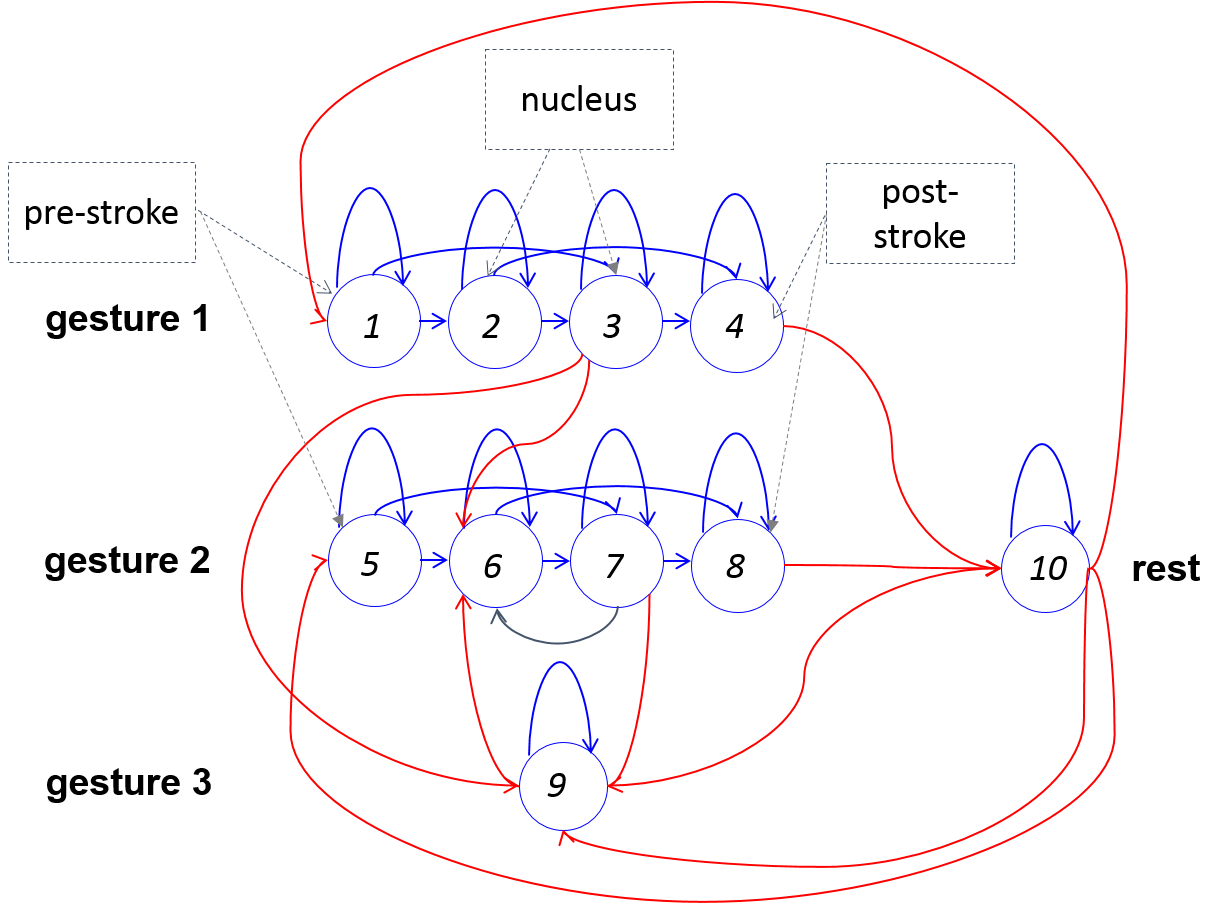
\includegraphics[width=0.7\columnwidth]{fig/combined_hmm.ps}
\caption{Combined HMM. The red lines are examples of new transitions combining
the HMMs.
Not all possible transitions are shown to avoid cluttering the diagram.}
\label{fig:combined}
\end{figure}

\subsection{Online Inference}
Once we have a trained model, we use fixed-lag smoothing \cite{murphy02} to do
online inference on the flattened HMM for real-time gesture recognition.
Fixed-lag smoothing is a modified forward-backward algorithm. Unlike online
filtering, which estimates the belief state at current time $t$ using forward
pass only, we estimate the state at $t - L$, given all the evidence up to the
current time $t$, i.e., compute $\gamma_{t - L}(s) \eqdef P(S_{t -
L} = s|\underline{x}_1^t)$, where $L>0$ is the lag. Introducing lag time is a
tradeoff between accuracy and responsiveness. Using some future evidence to
smooth the estimate can increase the accuracy while adding some delay. However
if the delay is small, it might be unnoticeable.
In the Experiment Evaluation section (Section~\ref{sec:evaluation}), we show
details about the relationship between $L$ and the recognition performance.

Fixed-lag smoothing can be implemented efficiently. We compute forward
probabilities $\alpha_t$ normally and keep a history window of $\alpha_{t -
L}\ldots\alpha_t$. At every time frame, we compute backward probabilities
$\beta$ from current time $t$ to $t - L$. Then we can compute
\begin{align}
\gamma_{t - L} = \alpha_{t - L} \cdot \beta_{t - L}
\end{align}  
The time complexity at each time frame is $O(N_s^2L)$ where $N_s$ is the total
number of hidden states in the flattened HMM. Note that at time $t$, the belief
state at $t - L$ is committed, while the belief state from $t - L + 1$ to $t$ will still be revised later.

We can then compute the most likely hidden state at $t - L$:
\begin{align}
\hat{s} = \arg\max_s \gamma_{t - L}(s)
\end{align}
We map the most likely hidden state to the gesture label it
belongs to (including the rest position) and the gesture phase. In this way
we achieve simultaneous segmentation and recognition.

Gesture events are detected at the boundary of a phase change: start pre-stroke,
start gesture nucleus and start post-stroke. This information, together with the
gesture label for the nucleus phase, are sent to the application level.

\begin{figure}[t]
\centering
\includegraphics[trim=0 5mm 0
5mm, clip, width=1.1\columnwidth]{fig/circle_shake_label.ps}
\caption{Most likely hidden states using fixed-lag smoothing. Different colors indicate different hidden states. Yellow indicates rest position.}
\label{fig:visual_hidden}
\end{figure}

Fig.~\ref{fig:visual_hidden} shows a visualization of the
most likely hidden states based on the online fixed-lag smoothing inference
with $L = 5$.
This is based on an input sequence of 6 gestures. The first 3 gestures are
``circle'' and the last 3 gestures are ``shake hand'' gestures. Notice that in
the first segment, at the beginning, the most likely hidden state is the
pre-stroke for ``shake hand'', but since we do not need to respond at this time,
the wrong estimate does not matter. After a few more frames, the estimates are
updated to have the correct most likely gesture label and the system
responds correctly when it detects the start of the post-stroke of ``circle''
gesture.

\section{Data Collection and User Study}
Previous related work does not appear to have gesture data sets
that include both gestures with distinct paths and gestures with distinct hand
poses. To evaluate our method, we collected a dataset with a vocabulary of 7
one-hand/arm gestures focusing on combining these two forms of gestures. They
are also chosen to span over different potential difficulties (see the comments in Table~\ref{tab:gestures}).

\begin{table}
\caption{List of gestures recorded in the dataset.}
\label{tab:gestures}
\centering
\begin{tabular}{|c|l|l|l|}
\hline
\# & Name of gesture & Form & Comment \\
\hline
1 & Swipe left & distinct path & simple path \\
\hline
2 & Swipe right & distinct path & simple path \\
\hline
3 & Circle & distinct path & complex path \\
\hline
4 & Horizontal wave & distinct path & has arbitrary repetitions \\
\hline
5 & Point & distinct hand pose & arbitrary path \\
\hline
6 & Palm forward & distinct hand pose & arbitrary path \\
\hline
7 & Grab & distinct hand pose & arbitrary path \\
\hline
\end{tabular}
\end{table}

The dataset contains data from 10 participants each
doing 4 sessions. All the participants are university students.
The participants were shown video demonstration of each gesture at the beginning. 

\subsection{Recording Setup and Procedure}
In each session, the participant stands at about 1.5m from the Kinect
for Windows sensor (version one), and performs each gesture 3 times
according to the text prompts on a screen indicating the name of the gesture to
perform.
The order of the gestures is random and the time between each gesture is random
(between 2s and 6s). The first 2 sessions have ``Rest'' prompts between each
gesture, telling participants to go to the rest position (hands relaxing at the
side of the body), and the second 2 sessions do not have ``Rest'' prompts so
participants can choose to rest or not between consecutive gestures. This too
distinguishes the dataset from previous ones \cite{Ruffieux2013, guyon13} where
gestures are always delimited by rest positions.

Unlike Ruffieux et al. \cite{Ruffieux2013}, we do not show video demonstration
every time the participants perform a gesture because we want a
realistic scenario. In real practice, it is unlikely that a user will follow a
video demonstration every time he/she does a gesture. The result of this is that
there will be more variations among the gestures.

To motivate movement for gestures with distinct hand poses that
require a continuous response, the text prompt asks participants to draw
random letters in the air with the specified hand pose. 

The full corpus contains $
10P \times 4S \times 7G \times 3R = 840$ gesture occurrences
where P = participants, S = sessions, G = unique gestures, R = repetitions per
gesture. There are approximately 96 minutes of continuous recording,
recorded in the raw data from the Kinect sensor, including RGB, depth and
skeleton data. Both the RGB and depth data have a resolution of
$640\times480$px. The frame rate is 30 frame per second (FPS).

\subsection{Qualitative Observations}
We find that there is considerable variations in the way participants perform
each gesture even they were given the same demonstration video. Major variations
are observed in speed, the magnitude of motion, the paths and hand poses.

For example, some participants do swipe left and right in a rather straight
horizontal line, while others have a more curved path. Some participants start
the circle gesture at the bottom, while others start at the top. Some
participants do swipe left and right with a palm forward pose while others have
less distinct hand poses (hand is more relaxed). However, within users, they are
quite consistent within each gesture. 

\subsection{User Preferences}
We did a survey with the participants with questions that can influence
gesture interface design. We asked them, given a gesture input interface:
\begin{itemize}
  \item Whether they prefer predefined gestures or user defined gestures: 90\%
  of the participants prefer to be able to define their own gestures if necessary while 10\% of them prefer to following prefined
gestures completely. As no one prefers to define their own gestures at the very
beginning either.
\item How to define gestures: 80\% prefer defining gesture by 
performing the gestures themselves; no one prefers to
define gestures solely via rules written in terms of positions and directions
of movement of the hands.
However 20\% prefer to being able to do both.
\item Number of repetitions per gesture for training: 50\% are willing to give a
maximum of 4 - 6 examples, 40\% are willing ot give 1 - 3 examples, and 10\% are
willing to give more than 13 examples. So average maximum is about 5
repetitions.
\item Number of gestures for an application: 80\% think 6-10 gestures are
appropriate and easy to remember for a given application, 20\% prefers 1 - 5
gestures.
\item Intuitiveness of the gesture vocabulary for PowerPoint presentation:
average score is 4 out of 5 where 5 is very intuitive.
\end{itemize}

\subsection{Implications for Gesture Interaction Interface}
Based on our observation of the large variation in gesture execution among
users and small variations within users, and the fact that a majority of
participants preferring defining their own gestures if they do not like the
predefined gestures, we suggest that it is more important to optimize user
dependent recognition. As no one prefers to define their own gesture at the very
beginning, it also means that having a reasonable predefined gesture set and
basic user independent model for recognition will be useful too.

Recognition methods based on examples will allow users to train models of their
own gestures easily. We also need to develop methods that
require relatively few training examples.

\section{Hybrid Performance Metric}
Both frame \cite{song12} and event-based \cite{guyon13} metrics has been
used for evaluating gesture recognition systems. A \textit{frame} is a
fixed-length, fixed-rate unit of time. It is often the smallest unit of measure
defined by the system \cite{ward11} and in such cases approximates continuous
time.
For example, in our case, a frame is a data frame consisting of a RGB data frame, a depth data frame and a skeleton data from the
sensor at 30 FPS. An \textit{event} is a variable duration sequence of frames
within a continuous time-series.  It has a start time and a stop time.

Each of these metrics alone may not be adequate for evaluating a real-time
gesture recognition system handling different types of gestures. Frame-based
evaluation is less relevant for gestures requiring discrete responses. For the ChaLearn Gesture Challenge 2012, Guyon et al.
\cite{guyon13} use the Levenshtein distance between the ordered list of
recognized events and the ground truth events. However, such event-based metrics
that ignore timing of recognition are inappropriate for real-time
applications where responsiveness of the system matters.

Ruffieux et al. combined a time-based metric with an event-based metirc
\cite{Ruffieux2013}. Ward et al. \cite{ward11} proposed a comprehensive
scheme of combining both frame and event scoring.
We believe that all three types of information -- frames, events and
timings -- are relevant for a real-time system that responds to different types
of gestures. Hence, we developed a hybrid performance metric.

For discrete flow gestures, the system responds at the end of the nucleus phase,
so the evaluation should be event-based. Let $T_{{\text{gt\_start\_pre}}}$ be
the ground truth start time of the pre-stroke phase and
$T_{{\text{gt\_stop\_post}}}$ be the ground truth stop time of the post-stroke
phase.
A recognized event is considered a true positive (TP) if the time of response ($T_{\text{response}}$) 
occurs between $T_{{\text{gt\_start\_pre}}}$ and $T_{{\text{gt\_stop\_post}}} +
0.5\times(T_{{\text{gt\_stop\_post}}} - T_{\text{gt\_start\_pre}})$. We allow
some margin for error because there can be small ground truth timing errors.
Once a TP event is detected, the corresponding ground truth event is not
considered for further matching, so that multiple responses for the same gesture
will be penalized. We then can compute event-based precision, recall and $F_1$
score.

For discrete flow gestures, we also define a Responsiveness Score (RS) as the
time difference in seconds between the moment when the system responds and the moment when the hand goes to a rest
position or changes gesture. Let $N_{TP}$ be the number of true positives, then
\begin{align}
RS = \frac{\sum_{i = 1}^{N_{TP}}T_{{\text{gt\_stop\_post}}} -
T_{\text{response}}}{N_{TP}}
\end{align}
A positive score means the responses are before the end of the post-strokes,
hence higher scores are better.

For continuous flow gestures, the system responds frame by frame,
so it is more appropriate to use frame-based evaluation. For all the frames that are
recognized as continuous gestures, we can compute the number of TPs by
comparing with the corresponding frame in the ground truth. Then, we can
compute frame-based precision, recall and $F_1$ score for all the frames
corresponding to continuous flow gestures.

The average of the two $F_1$ scores gives an indication of the overall system
performance.

\section{Experiment Evaluation}\label{sec:evaluation}
\begin{figure}[t]
\centering
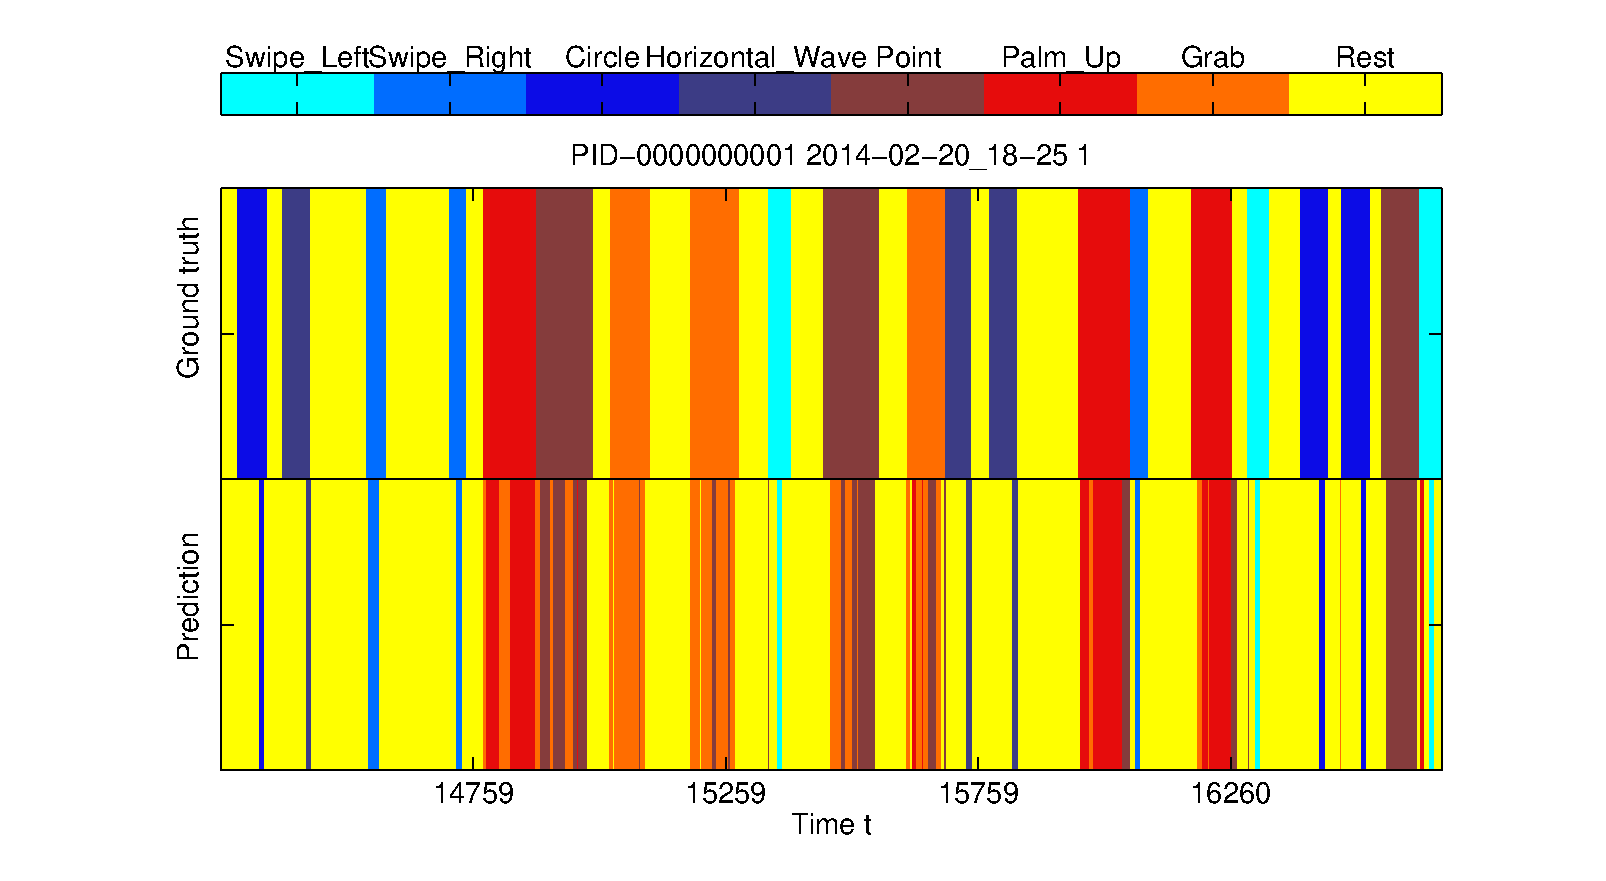
\includegraphics[trim=10mm 5mm 10mm 5mm, clip,
width=\columnwidth]{fig/recog_result_m3.eps}
\caption{Comparison between recognition result using online inference
and ground truth.
The colors correspond to different gestures. For discrete flow gestures
(swipe left/right, circle, horizontal wave), one color segment with a fixed
length is shown at the time of response. For continuous flow gestures, the
recognized gesture is shown at each frame indicating frame-by-frame responses.}
\label{fig:recog-result}
\end{figure}
We evaluate our method based on the dataset we collected, using the
evaluation metrics proposed in the previous section. The evaluation is based
on the assumption that all the gestures with distinct paths (gesture \#1--4)
are discrete flow gestures, and gestures with distinct hand poses (gesture
\#5--7) are continuous flow gestures. 

Our survey results show that it is
important to allow users to quickly define and train their own gestures. Hence,
we evaluate our system using user dependent training and testing. For each user
in the dataset, we use the first 2 sessions of recording (6 samples per gesture)
as training examples, and the last 2 sessions as testing examples.
Fig.~\ref{fig:recog-result} shows a visualization of the recognition result on a
test sequence. The figure highlights the challenges in the test sequences:
there are 21 gestures in each continuous unsegmented sequence; sometimes
gestures immediately follow one another. We report the average results for 10 users.

\begin{table}[t]
\caption{Results from using different topologies. The numbers in parentheses are
standard deviations. The results are based on using 3 mixtures of Gaussians
for all hidden states, and lag time
$L = 5$ frames.}
\label{tab:result}
\centering
\begin{tabular}{|l|l|p{1.8cm}|p{1.8cm}|}
\hline
& & Same topology for two \textit{forms} of gestures & Different
topologies for two \textit{forms} of gestures \\
\hline
\multirow{4}{2cm}{Path \& discrete flow gestures} 
& Precision & 0.77 (0.14) & 0.77 (0.15) \\
\cline{2-4}
& Recall & 0.89 (0.09) & 0.88 (0.11)\\
\cline{2-4}
& $F_1$ & 0.82 (0.10) &  0.81 (0.11)\\
\cline{2-4}
& Responsiveness (s) & 0.6 (0.3) & 0.6 (0.3) \\
\hline
\multirow{4}{2cm}{Pose \& continuous flow gestures}
& Precision & 0.54 (0.13) & 0.60 (0.10) \\
\cline{2-4}
& Recall & 0.24 (0.08) & 0.62 (0.09) \\
\cline{2-4}
& $F_1$ & 0.33(0.09) & 0.61 (0.09) \\
\hline
\textbf{Average} & $F_1$ & 0.58 (0.10) & \textbf{0.71 (0.10)} \\
\hline
\end{tabular}
\end{table}

\begin{itemize}
  \item \textbf{Compare different topologies: }
We compare our unified framework with a common HMM-based approach
used in previous works~\cite{sharma00, Starner95}, i.e., using the same
left-right topology for all gestures. Table~\ref{tab:result} compares the results between the two methods.
The third column is the result from treating the two \textit{forms} of gestures
in the same way, i.e., all gestures have the same left-right Bakis model for their nucleus
phases. The forth column is the result from using a left-right Bakis model for
path gestures and a single state for pose gestures. To have a fair comparison,
all hidden states have 3 mixtures of Gaussians. The result 
shows that our method of having different HMM topologies for the two
\textit{forms} of gestures significantly increases the precision, the recall and
the $F_1$ score for pose gestures.

\item \textbf{Compare different lag times: }
Using our unified framework, we investigated how the $F_1$ scores change with
respect to the lag time ($L$) in fixed-lag smoothing (Fig.~\ref{fig:lag}). The
performance increases as $L$ increases, and plateaus at $L=8$ frames which is about 0.3s at 30 FPS. This shows that more evidence does help to smooth the estimates until a limit, and we do not need to sacrifice too much delay to reach the limit. Our result shows that the
responsiveness score stays around 0.6-0.7 seconds as we increase $L$.

\begin{figure}[t]
\centering
\includegraphics[trim=0 5mm 0 15mm, clip, width=\columnwidth]{fig/f1_lag.ps}
\caption{$F_1$ scores versus lag time.}
\label{fig:lag}
\end{figure}

\begin{figure}[t]
\centering
\includegraphics[trim=10mm 5mm 10mm 15mm,
clip, width=\columnwidth]{fig/f1_nM.ps}
\caption{$F_1$ scores versus number of mixtures of Gaussians. Lag time
$L = 5$ frames.}
\label{fig:mixtures}
\end{figure}

\item \textbf{Compare different number of mixtures:}
Within a user, there may be variation in the hand pose for a
gesture with distinct hand pose. For example, the ``point'' hand pose can have
different orientations. This is why we use a mixture of Gaussians for the
emission probabilities. Fig.~\ref{fig:mixtures}
shows that the $F_1$ scores increases as the number of mixtures (M) increases
until $M=3$.
After that, we start to see the effect of overfitting. Then, we experimented
with using different $M$'s for path and pose gestures. We set $M^\text{path} =
3$ for path gestures, and use a different $M^{\text{pose}}_g\in \{3\ldots6\}$ for pose gesture $g$. Each
$M^{\text{pose}}_g$ is chosen using Bayesian Information
Criterion~\cite{fraley06}. Using this method, we are able to improve 
the overall average $F_1$ score to 0.81 when $L=8$ frames.

\end{itemize}

Our system is fast to train and extensible. The average computation time
for training the model for one user is about 5s with 7 gestures and 6 training examples per
gesture. New gestures can be added by recording 3-6 repetitions of
the gesture using the Kinect; the system will train an HMM model for the gesture
and add it to the existing combined HMM. This process takes only a few minutes.

We also evaluated our method
with a public dataset (ChAirGest) containing 10 path gestures performed by 10
users~\cite{yin13}. We obtained an $F_1$ score of 0.86 with
offline user independent recognition. While it
offers a baseline only for path gestures, it does show that our unified approach
performs at the state of the art on this category of gesture.

% An example of a floating figure using the graphicx package.
% Note that \label must occur AFTER (or within) \caption.
% For figures, \caption should occur after the \includegraphics.
% Note that IEEEtran v1.7 and later has special internal code that
% is designed to preserve the operation of \label within \caption
% even when the captionsoff option is in effect. However, because
% of issues like this, it may be the safest practice to put all your
% \label just after \caption rather than within \caption{}.
%
% Reminder: the "draftcls" or "draftclsnofoot", not "draft", class
% option should be used if it is desired that the figures are to be
% displayed while in draft mode.
%

% Note that IEEE typically puts floats only at the top, even when this
% results in a large percentage of a column being occupied by floats.


% An example of a double column floating figure using two subfigures.
% (The subfig.sty package must be loaded for this to work.)
% The subfigure \label commands are set within each subfloat command, the
% \label for the overall figure must come after \caption.
% \hfil must be used as a separator to get equal spacing.
% The subfigure.sty package works much the same way, except \subfigure is
% used instead of \subfloat.
%
%\begin{figure*}[!t]
%\centerline{\subfloat[Case I]\includegraphics[width=2.5in]{subfigcase1}%
%\label{fig_first_case}}
%\hfil
%\subfloat[Case II]{\includegraphics[width=2.5in]{subfigcase2}%
%\label{fig_second_case}}}
%\caption{Simulation results}
%\label{fig_sim}
%\end{figure*}
%
% Note that often IEEE papers with subfigures do not employ subfigure
% captions (using the optional argument to \subfloat), but instead will
% reference/describe all of them (a), (b), etc., within the main caption.

% Note that IEEE does not put floats in the very first column - or typically
% anywhere on the first page for that matter. Also, in-text middle ("here")
% positioning is not used. Most IEEE journals/conferences use top floats
% exclusively. Note that, LaTeX2e, unlike IEEE journals/conferences, places
% footnotes above bottom floats. This can be corrected via the \fnbelowfloat
% command of the stfloats package.

\section{Conclusion and Future Work}
We designed our system from natural human computer interaction perspective.
The evaluation shows promising results for the unified probabilistic
recognition framework that handles two \textit{forms}
of gestures seamlessly.
Even using only a small number of training examples (e.g. 6 per gesture), our
system can achieve an average $F_1$ score of 0.81 for two \textit{forms} of
gestures.
Using the framework, we developed a real-time (30 FPS) gesture controlled
presentation application similar to the one described at the beginning of this paper.

The performance for pose gestures is lower than that
for path gestures. This may be due to limit in
both the pixel and the depth resolutions of the Kinect sensor. It would be interesting to test
the new version of the Kinect sensor which uses a time-of-flight depth sensor
and is reported to have a higher resolution. We are also going to to explore
other feature descriptors and encoding methods to see whether we can
improve the result for pose gestures.

Using embedded training and hidden state information, we can effectively
detect gesture phases, allowing the system to respond more promptly. On average,
for discrete flow gestures, the system responds 0.6s before the hand comes to
rest. 

We collected a new dataset that includes two \textit{forms} of gestures, a
combination currently lacking in the community, and plan to make it
public. We have also proposed a hybrid evaluation metric
that is more relevant to real-time interaction and different types of gestures.
 
% use section* for acknowledgement

% trigger a \newpage just before the given reference
% number - used to balance the columns on the last page
% adjust value as needed - may need to be readjusted if
% the document is modified later
%\IEEEtriggeratref{8}
% The "triggered" command can be changed if desired:
%\IEEEtriggercmd{\enlargethispage{-5in}}

% references section

% can use a bibliography generated by BibTeX as a .bbl file
% BibTeX documentation can be easily obtained at:
% http://www.ctan.org/tex-archive/biblio/bibtex/contrib/doc/
% The IEEEtran BibTeX style support page is at:
% http://www.michaelshell.org/tex/ieeetran/bibtex/
\bibliographystyle{IEEEtran}
% argument is your BibTeX string definitions and bibliography database(s)
\bibliography{IEEEabrv,main}
%
% <OR> manually copy in the resultant .bbl file
% set second argument of \begin to the number of references
% (used to reserve space for the reference number labels box)
% \begin{thebibliography}{1}
% 
% \bibitem{IEEEhowto:kopka}
% H.~Kopka and P.~W. Daly, \emph{A Guide to \LaTeX}, 3rd~ed.\hskip 1em plus
%   0.5em minus 0.4em\relax Harlow, England: Addison-Wesley, 1999.
% 
% \end{thebibliography}

% that's all folks
\end{document}


